\section{The best Gaussian state and the resolution gap}
\label{sec:best}

From now on we consider flows with one degree of freedom, $f = (p, g(q))$, that is, $H = p^2/2 + V(q)$ with $g = -V'$. Their strain is $a(q)\,\mathrm{diag}(1,-1)$ in the coordinates $(v,w)$ of Sec.~\ref{sec:decomposition}, with $a$ from Eq.~\eqref{eq:stretch}. We write $T = S + \sigma^2 I$ for the covariance of $Y$ and use $(v,w)$ components.

\begin{lemma}[Gaussian states of one-degree-of-freedom flows]
\label{lem:lambdaphi}
For $\rho_t = \mathcal N(m,S)$,
\begin{equation}
R = \lambda\,\varphi, \qquad \lambda = \E_{\rho_t}[a(X_q)], \qquad \varphi = \frac{T_{ww} - T_{vv}}{T_{ww} + T_{vv}} .
\label{eq:lambdaphi}
\end{equation}
\end{lemma}

\begin{proof}
By Theorem~\ref{thm:gaussian}, $R = \tr(F\bar G)/\tr F$ with $\bar G = \lambda\,\mathrm{diag}(1,-1)$ and $F = T^{-1}$. For a $2\times2$ matrix, $F_{vv} = T_{ww}/\det T$ and $F_{ww} = T_{vv}/\det T$.
\end{proof}

The two factors in Eq.~\eqref{eq:lambdaphi} are the two requirements of Sec.~\ref{sec:gaussian}: $\lambda$ is the strain felt by the state and $\varphi \in (-1,1)$ is the anisotropy of the observer's focus. The aspect factor $\varphi$ depends on $S$ only through $S_{vv}$ and $S_{ww}$, while $\lambda$ depends on $S$ through the variance $S_{qq} = (S_{vv} + 2S_{vw} + S_{ww})/2$ of $X_q$. At fixed $S_{vv}, S_{ww}$, $S_{qq}$ is smallest when $S_{vw} = -\sqrt{S_{vv}S_{ww}}$, a state of zero width: a straight segment whose direction is tilted from $w$ towards $-v$. If $\lambda$ decreases with $S_{qq}$, which is the case at the point of maximal strain, the supremum over Gaussian states is approached by states that tend to a segment of zero width; we admit such degenerate Gaussian states as limits and call them segments. Writing $x = \sqrt{2S_{qq}}$, which for a nearly $w$-aligned segment is close to its standard deviation along its length, the remaining optimization over the tilt can be done in closed form (Appendix~\ref{app:best}):
\begin{equation}
\max_{\text{tilt}}\varphi = \frac{x}{\sqrt{x^2 + 4\sigma^2}} .
\label{eq:phimax}
\end{equation}
This reduces the best Gaussian state to a maximization over one variable.

\begin{theorem}[Pendulum]
\label{thm:pendulum}
For the pendulum, $a(q) = (1-\cos q)/2$ and $\kappa = 1$. For every $\sigma > 0$ the supremum of $R$ over Gaussian states is
\begin{equation}
R^*(\sigma) = \sup_{x > 0}\;\frac{1 + e^{-x^2/4}}{2}\,\frac{x}{\sqrt{x^2 + 4\sigma^2}} .
\label{eq:Rstar}
\end{equation}
For $\sigma \leq \sigma_c = 0.93909\ldots$ it is attained at a finite $x$, by a zero-width segment centred at $q = \pi$, with standard deviation along its length close to $2\sqrt\sigma$, tilted from $w$ towards $-v$ by an angle close to $\sigma/4$. Its gap has the expansion
\begin{align}
1 - R^*(\sigma) &= \sigma - \frac78\sigma^2 + \frac{65}{96}\sigma^3 - \frac{61}{128}\sigma^4 \nonumber\\
&\quad + \frac{3151}{10240}\sigma^5 - \frac{8483}{46080}\sigma^6 + O(\sigma^7) .
\label{eq:series}
\end{align}
For $\sigma > \sigma_c$, $R^*(\sigma) = 1/2$ and is not attained.
\end{theorem}

The proof is in Appendix~\ref{app:best}. The coefficients in Eq.~\eqref{eq:series} were computed in exact rational arithmetic up to $\sigma^{11}$; the truncation error of the series equals the size of the next term, and through $\sigma^{11}$ it reproduces Eq.~\eqref{eq:Rstar} to $10^{-9}$ at $\sigma = 0.3$ (Fig.~\ref{fig:best}).

\begin{figure*}[t]
\centering
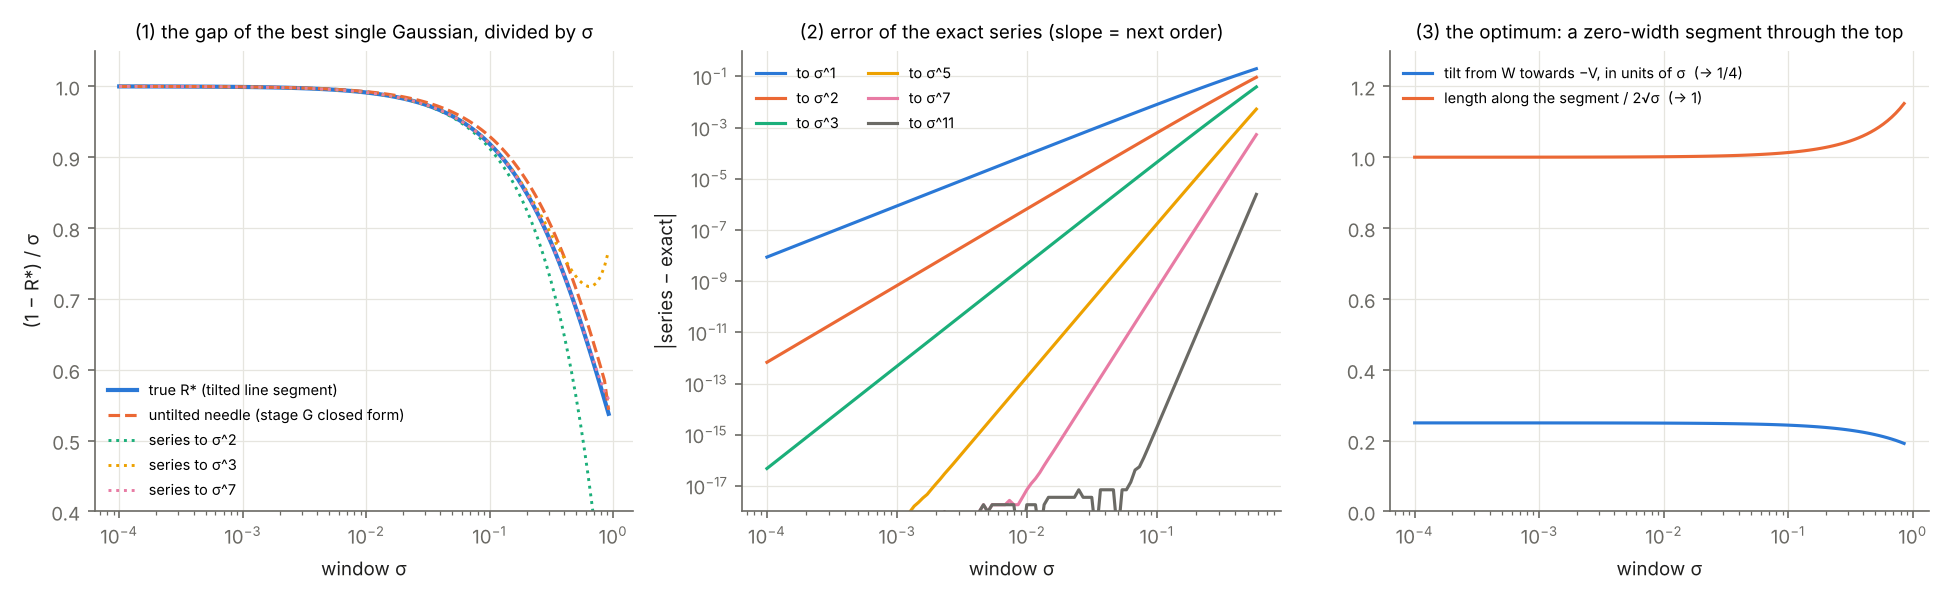
\includegraphics[width=0.95\textwidth]{figures/fig2_best_gaussian.png}
\caption{Best Gaussian state of the pendulum. (1) Gap $(1-R^*)/\sigma$ of the optimal tilted segment, of the untilted needle, and of truncations of the series~\eqref{eq:series}. (2) Error of the truncated series; the slope equals the next order. (3) Shape of the optimum: tilt from $w$ towards $-v$ in units of $\sigma$ ($\to1/4$) and length in units of $2\sqrt\sigma$ ($\to1$).}
\label{fig:best}
\end{figure*}

For a strain that is exactly quadratic about its maximum the optimization can be done completely.

\begin{theorem}[Quadratic strain]
\label{thm:quadratic}
Let $a(q) = \kappa - b(q - q_*)^2$ with $\kappa, b > 0$, and let $\varepsilon = \sigma\sqrt{b/\kappa}$. Among Gaussian states with $\varphi \geq 0$,
\begin{equation}
\frac{R^*}{\kappa} = \left(1 - \frac{\varepsilon\nu}{2}\right)\sqrt{\frac{\nu}{\nu + 4\varepsilon}},
\qquad \nu = \sqrt{4 + 9\varepsilon^2} - 3\varepsilon ,
\label{eq:quadratic}
\end{equation}
attained by the zero-width segment centred at $q_*$ with $S_{qq} = \tfrac12\sigma\nu\sqrt{\kappa/b}$. In particular $1 - R^*/\kappa = 2\varepsilon - \tfrac52\varepsilon^2 + \tfrac74\varepsilon^3 - \tfrac18\varepsilon^4 - \tfrac{53}{64}\varepsilon^5 + O(\varepsilon^6)$.
\end{theorem}

The restriction $\varphi \geq 0$ selects states whose focus is sharper across $v$ than across $w$, the relevant ones near a maximum of $a$. It is needed because for such polynomial potentials $|a|$ is unbounded and the global strain rate is infinite; here $\kappa$ denotes the maximum of $a$, not the supremum of $|a|$. The double well $g = q - q^3$ ($a = 1 - \tfrac32 q^2$) and the quartic oscillator $g = -q^3$ ($a = \tfrac12 - \tfrac32q^2$) are exactly of this form. Both theorems share the same leading behaviour, which we state for a general maximum.

\begin{proposition}[Resolution gap of Gaussian states]
\label{prop:gap}
Let $a$ be of at most polynomial growth and four times continuously differentiable near a non-degenerate maximum $\kappa = a(q_*) > 0$ with $a''(q_*) = -2b$, and let $\beta = b/2$, the rate at which the strain decreases quadratically along the contracting direction $w$ through the maximum. Let $R^*(\sigma)$ be the supremum of $R$ over Gaussian states with $\varphi \geq 0$. Then
\begin{equation}
\kappa - R^*(\sigma) \leq 2\sqrt{2\beta\kappa}\,\sigma + O(\sigma^2) .
\label{eq:gap}
\end{equation}
Equality holds to this order whenever $\E_\rho[a(X_q)] \leq \Lambda(S_{qq})$ for all Gaussian states $\rho$ with $\varphi \geq 0$, for a non-increasing function $\Lambda$ with $\Lambda(s) = \kappa - bs + O(s^2)$ as $s \to 0$ and $\sup_{s \geq s_0}\Lambda(s) < \kappa$ for every $s_0 > 0$. This condition holds for the pendulum, with $\Lambda(s) = (1 + e^{-s/2})/2$, $\beta = 1/8$ and coefficient $1$, and for quadratic strain (Theorem~\ref{thm:quadratic}).
\end{proposition}

The proof (Appendix~\ref{app:best}) balances two losses. A segment with standard deviation $x$ along its length loses $\tfrac12 b x^2$ of strain because its ends leave the maximum, and loses a fraction $2\sigma^2/x^2$ of focus because the window has width $\sigma$. The sum $\tfrac12 b x^2 + 2\kappa\sigma^2/x^2$ is smallest for $x^2 = 2\sigma\sqrt{\kappa/b}$, where both losses equal $\sqrt{2\beta\kappa}\,\sigma$. The gap is linear in $\sigma$, although the window enters the loss of focus quadratically, because the optimal length grows like $\sqrt\sigma$.

Figure~\ref{fig:flows} (panel 1) shows the gap for four flows: the pendulum and the double well and quartic oscillator, which are covered by Theorems~\ref{thm:pendulum} and~\ref{thm:quadratic}, and the twist flow $H = \tfrac12\ln(1+q^2+p^2)$. The numerically optimized Gaussian states agree with $2\sqrt{2\beta\kappa}$ to $10^{-7}$ after extrapolation to $\sigma\to0$: coefficients $1$, $\sqrt6$, $\sqrt3$ and $\sqrt3/2$. The twist flow is not of the form $f = (p,g(q))$: its maximal strain $\kappa = 1/4$ is attained on the circle $q^2+p^2 = 1$, and its stretching direction rotates along the contracting direction. For it, $\beta = 3/8$ is the sum of the decrease of the strain with radius ($1/8$) and of the turning of the stretching direction ($1/4$). Proposition~\ref{prop:gap} is proved here only for $f = (p,g(q))$; the twist flow is a numerical observation.
